\section{Ruteo}

Realice el ruteo de los siguientes programas e indique qué es lo que imprimen. Cada vez que el valor de una variable cambie, escríbalo en una nueva fila de la tabla. Recuerde que si una variable es de tipo string, debe colocar su valor entre comillas simples ’ ’.

\begin{figure}[H]
    \centering
    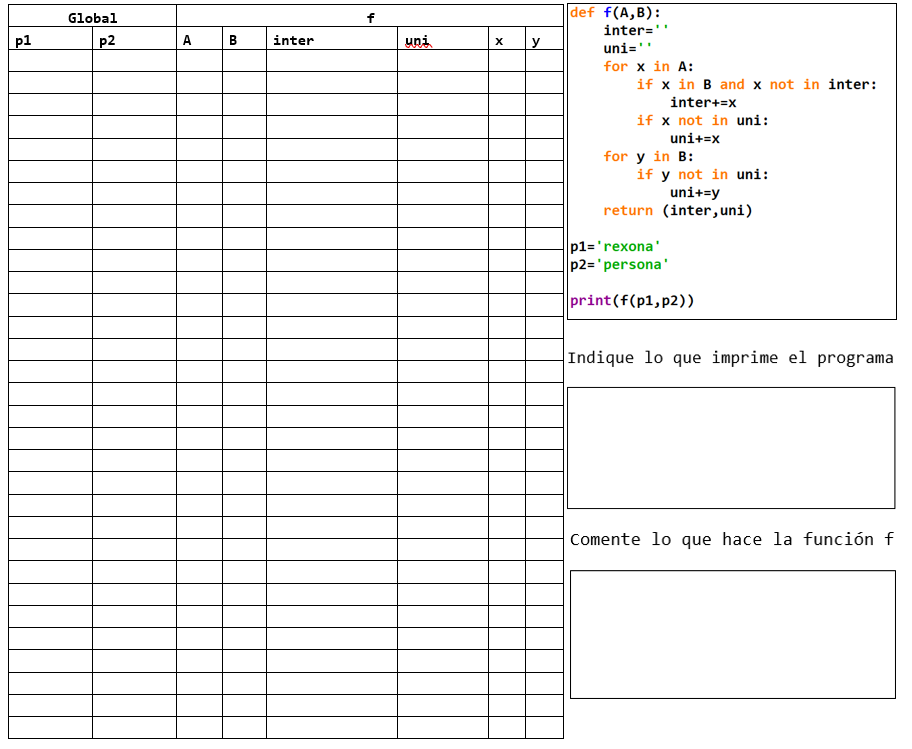
\includegraphics[scale=0.9]{Guia/ruteo1.png}    
\end{figure}